%---------------------------------------------------------------------
%
%                          Cap�tulo 4
%
%---------------------------------------------------------------------
%
% 04Imagenes.tex
% Copyright 2009 Marco Antonio Gomez-Martin, Pedro Pablo Gomez-Martin
%
% This file belongs to the TeXiS manual, a LaTeX template for writting
% Thesis and other documents. The complete last TeXiS package can
% be obtained from http://gaia.fdi.ucm.es/projects/texis/
%
% Although the TeXiS template itself is distributed under the 
% conditions of the LaTeX Project Public License
% (http://www.latex-project.org/lppl.txt), the manual content
% uses the CC-BY-SA license that stays that you are free:
%
%    - to share & to copy, distribute and transmit the work
%    - to remix and to adapt the work
%
% under the following conditions:
%
%    - Attribution: you must attribute the work in the manner
%      specified by the author or licensor (but not in any way that
%      suggests that they endorse you or your use of the work).
%    - Share Alike: if you alter, transform, or build upon this
%      work, you may distribute the resulting work only under the
%      same, similar or a compatible license.
%
% The complete license is available in
% http://creativecommons.org/licenses/by-sa/3.0/legalcode
%
%---------------------------------------------------------------------

\chapter{Implementaci\'on y Especificaci\'on}
\label{cap4}
\label{cap:implentacion-especificacion}


\begin{FraseCelebre}
\begin{Frase}
%El alma nunca piensa sin una imagen mental.
\end{Frase}
\begin{Fuente}
%Arist�teles
\end{Fuente}
\end{FraseCelebre}

%-------------------------------------------------------------------
\section{Introducci\'on}
%-------------------------------------------------------------------
\label{cap4:sec:intro}

Una vez decididas las herramientas que se iban a usar y con gran parte de la informaci\'on recogida, lleg\'o el momento de realizar un an\'alisis del funcionamiento de Android y dise\~nar un protocolo de red que ayudase a conectar la aplicaci\'on de Android con el juego de Unity. En este cap\'itulo se explicar\'an todas las decisiones que se tomaron a la hora de implementar ambas aplicaciones y se ampliar\'a la informaci\'on sobre como interactuan ambos sistemas.

%-------------------------------------------------------------------
\section{Arquitectura global}
%-------------------------------------------------------------------
\label{cap4:sec:global}

Tal y como se ha planteado en los anteriores cap\'itulos, para la realizaci\'on de este proyecto se ha requerido de la conexi\'on entre una aplicaci\'on de escritorio realizada con Unity3D y una aplicaci\'on de un dispositivo m\'ovil Android. Ambos dispositivos recibir\'an y enviaran mensajes pero el protocolo a seguir ha sido UDP. UDP es un protocolo a nivel de transporte que permite el env\'io de datagramas a trav\'es de la red sin necesidad de haber realizado una conexi\'on previa. Esto se consigue gracias a que la cabecera del propio datagrama UDP incorpora la informaci\'on suficiente para realizar su direccionamiento.
\\
Con la utilizaci\'on de UDP se corre el riesgo de p\'erdida de informaci\'on, cosa que para este proyecto es menos probable ya que en ning\'un momento este datagrama sale a internet. Se ha puesto como requisito que tanto el ordenador como el dispositivo m\'ovil se encuentren conectados a la misma red local, lo que hace muy poco probable la p\'erdida de paquetes UDP. Esta posible p\'erdida ser\'a analizada en el cap\'itulo siguiente donde se analiza las pruebas realizadas con usuarios.
\\


A la hora de iniciar la conexi\'on, es la aplicaci\'on m\'ovil la que va a conectarse al puerto que abra la aplicaci\'on de escritorio previamente. Para poder hacer esto, se propuso la utilizaci\'on de un QR. Este QR contiene la informaci\'on de la IP del ordenador donde se est\'a ejecutando el juego y el puerto designado para la recepci\'on de los mensajes provenientes de la aplicaci\'on m\'ovil. Una vez la aplicaci\'on m\'ovil guarda esos datos extraidos tras leer el c\'odigo QR, se incia la conexi\'on y el intercambio de paquetes entre ambas aplicaciones.
\\
La decisi\'on de usar UDP cobr\'o su importancia en este apartado ya que no se espera un intercambio ordenado de informaci\'on entre ambas aplicaciones ,ya que el usuario puede hacer una pulsaci\'on en la pantalla del m\'ovil en cualquier momento. La informaci\'on que se env\'ia desde la aplicaci\'on Android es la siguiente:

\begin{enumerate}

\item Dimensiones de la pantalla del dispositivo m\'ovil con 2 enteros, ancho y alto.
\item Pulsaci\'on en la pantalla con 3 enteros (X, Y, tipo de evento). 

\end{enumerate}

Las dimensiones se mandan \'unicamente una vez al iniciar la conexiones mientras que las coordenadas de las pulsaciones se env\'ian cada vez que estas ocurren. El tercer entero que se manda en estos paquetes viene definido por cada tipo de pulsaci\'on que se puede registrar en Android. Los tipos contemplados son:
\begin{itemize} 
\item \textbf{ACTION\_DOWN:} Env\'ia el valor 0. Este evento se dispara al realizar una pulsaci\'on en la pantalla.
\item \textbf{ACTION\_UP:} Env\'ia el valor 2. Este evento se dispara al levantar el dedo de la pantalla.
\end{itemize}

En el lado del servidor de la aplicaci\'on de Unity se espera la llegada de las dimensiones de la pantalla que env\'ia la aplicaci\'on m\'ovil para enviar desde su lado la siguiente informaci\'on en paquetes diferentes:

\begin{enumerate}
\item Tiempo de vibraci\'on que debe realizarse cada vez que se pulse una posici\'on correcta de la pantalla del m\'ovil. Se considera una pulsaci\'on correcta un punto que est\'e dentro de un bot\'on.
\item Imagen del mando con o sin fondo cogido directamente de una c\'amara de Unity.
\item En caso de que el juego admita la vibraci\'on del m\'ovil, se env\'ia la acci\'on de realizar la vibraci\'on o no.
\end {enumerate}

El primero de estos mensajes con el tiempo de vibraci\'on solamente se env\'ia una \'unica vez al inicio de la conexi\'on.
\\
El flujo de mensajes durante la ejecuci\'on de estas aplicaciones tiene un intercambio de datagramas constante de \'ordenes para que el dispositivo m\'ovil vibre, im\'agenes compridas y coordenadas de pulsaciones de la pantalla del dispositivo m\'ovil.
La figura XXXX describe este protocolo de manera m\'as gr\'afica.

\begin{figure}[h]
\centering
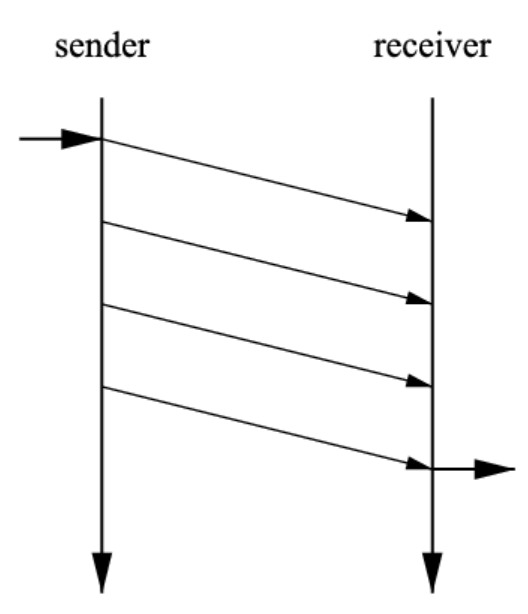
\includegraphics[width=0.6\textwidth]{Imagenes/Bitmap/UDP-protocol.png}
\caption{Protocolo de comunicaci\'on entre las aplicaciones}
\label{Protocolo Android - Unity}
\end{figure}

\newpage
%-------------------------------------------------------------------
\section{Aplicaci\'on m\'ovil}
%-------------------------------------------------------------------
\label{cap4:sec:android}

La principal funci\'on de este proyecto es el uso de un dispositivo Android para controlar de manera remota un videojuego realizado en Unity. Para esto es necesario conocer la arquitectura de Android y c\'omo funciona el ciclo de vida de sus aplicaciones.
La siguiente figura muestra el ciclo de vida de cualquier aplicaci\'on que se ejecute en un dispositivo Android.
\\
\begin{figure}[h]

\centering
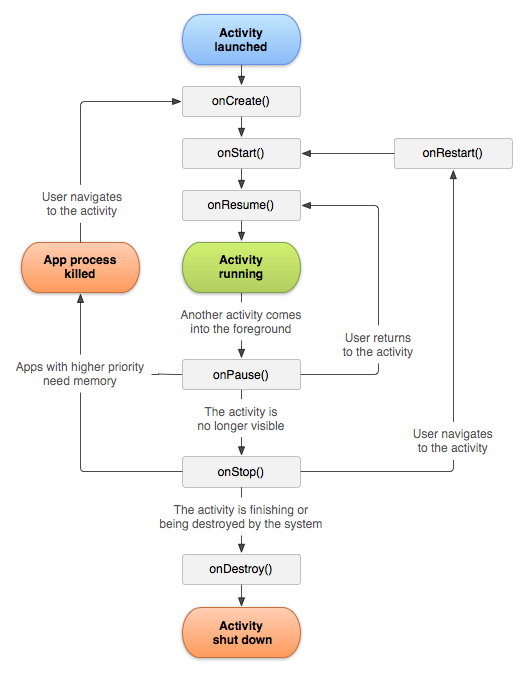
\includegraphics[width=0.6\textwidth]{Imagenes/Bitmap/Ciclo_de_vida_Android.png}
\caption{Ciclo de Vida de una Actividad de Android}
 \label{Ciclo de vida android}
\end{figure}
\\
Como puede observarse, cada Activity de una aplicaci\'on ejecutada en Android tiene varias etapas por las que puede pasar:

\begin{enumerate}
\item onCreate()
\item onStart()
\item onResume()
\item onPause()
\item onStop()
\item onDestroy()
\end {enumerate}

Cuando el usuario comienza a abandonar la actividad, el sistema llama a m\'etodos para desmantelarla. En algunos casos, este desmantelamiento es solo parcial ya que la actividad todav\'ia reside en la memoria (por ejemplo, cuando el usuario cambia a otra app) y a\'un puede volver al primer plano. En caso de que el usuario vuelva a poner dicha actividad en primer plano, esta se reanuda donde el usuario la dej\'o.
\\
Adem\'as de ciclo de vida, Android tiene un sistema de permisos. Desde la versi\'on 6.0 de Android (nivel de API 23) pueden incluirse en el fichero de manifiesto de la app los permisos que se deben solicitar al usuario para poder acceder a algunos recursos espec\'ificos. En este proyecto se necesita usar la c\'amara para poder realizar la lectura del c\'odigo QR, es por esto que se ha tenido que a\~nadir este permiso en el fichero de manifiesto de la app.
\\
Este c\'odigo QR es generado gracias a la librer\'ia de ZXing.NET desde la aplicaci\'on de Unity, la cual se cuenta en la siguiente secci\'on. Android por su parte incorpora una API para la lectura de c\'odigos. El c\'odigo QR contiene la siguiente informaci\'on:

\begin{itemize}
\item IP del servidor donde se est\'a ejecutando el juego.
\item Puerto de escucha del servidor.
\end {itemize}

Si el c\'odigo QR que se lee es correcto, se lanza una segunda Activitidad. La creaci\'on de una segunda actividad permite usar un archivo de manifiesto diferente y con \'el, generar una interfaz de usuario adecuada a esta segunda actividad. Esta segunda actividad tiene como prop\'osito establecer la comunicaci\'on con el servidor ya iniciado en la direcci\'on IP extraida del c\'odigo QR y a su vez el intercambio de informaci\'on (pulsaciones e im\'agenes) durante la sesi\'on de juego.
\\
\begin{figure}[h]
\centering
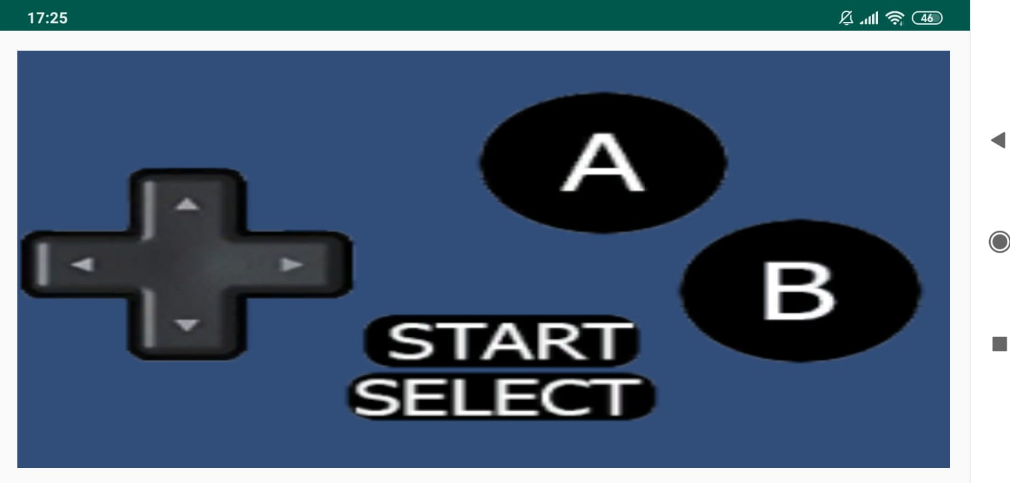
\includegraphics[width=0.8\textwidth]{Imagenes/Bitmap/Mando.png}
\caption{Vista del mando enviado desde Unity a Android}
 \label{Mando}
\end{figure}
\\
En caso de que el c\'odigo QR se lea correctamente, se inciar\'a la conexi\'on con el servidor que se est\'a ejecutando en Unity. En el siguiente apartado se explica la ejecuci\'on en la lado de Unity y el inicio de la conexi\'on con este. Desde Unity se env\'ia de manera constanste un streaming de im\'agenes sacadas de una c\'amara auxiliar colocada en la escena del juego. Esto permite en el env\'io de tanto un mando, mando con gameplay o \'unicamente gameplay. Para la demostraci\'on de este proyecto, se ha optado por el env\'io de la im\'agen de un mando de manera exclusiva. Este mando puede verse en la figura XXXXX . 
\\

Esta im\'agen llega al dispositivo Android tras realizarse una compresi\'on a formato PNG en el lado del servidor. Este array de bytes que llega es convertido a un tipo Bitmap mediante \textit{BitmapFactory} y es usado como fondo de la Actividad. Este proceso se realiza constantemente ya que en caso de que se quiera utilizar para gameplay, este requiere de fluidez. En el cap\'itulo siguiente se tratan las pruebas con usuario donde se hace un estudio de cu\'anto tarda esta im\'agen en procesarse. 
\\
La arquitectura de este proyecto de Android puede verse en la figura XXXX. 
\\
\begin{figure}[h]
\centering
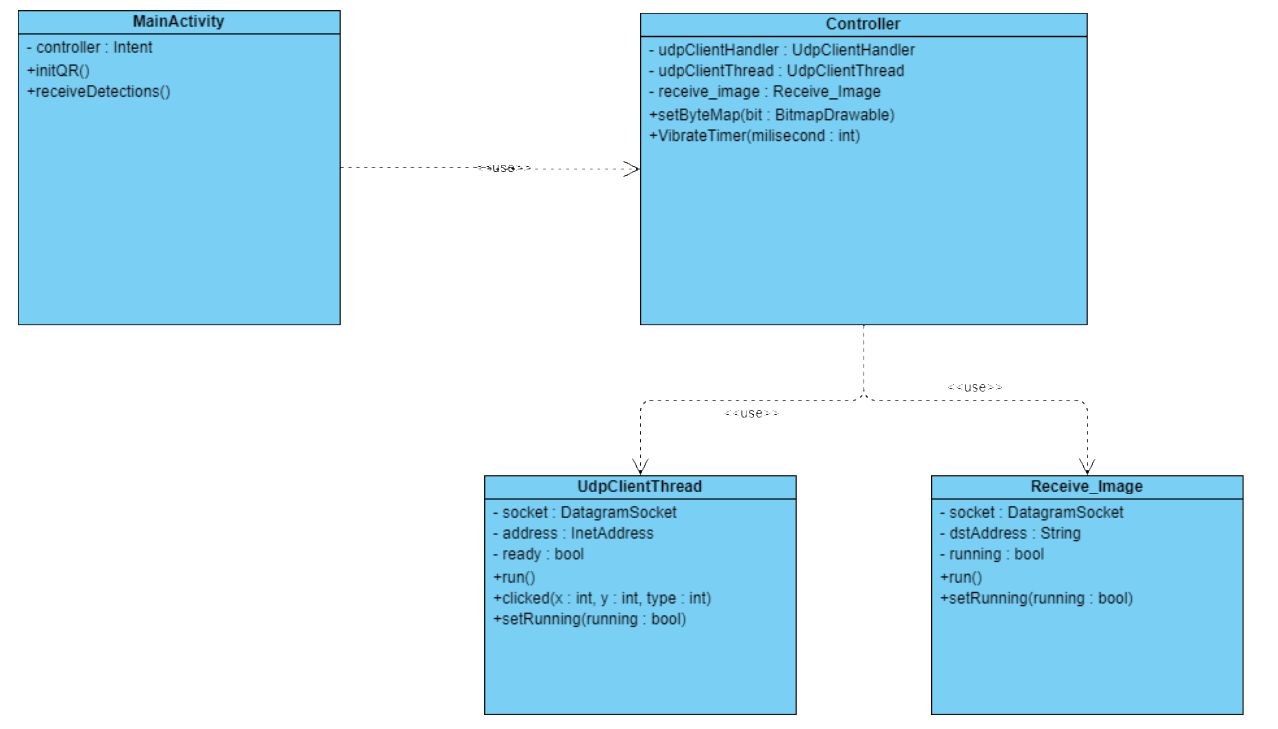
\includegraphics[width=1.0\textwidth]{Imagenes/Bitmap/Arquitectura_Android.png}
\caption{Arquitectura de la aplicaci\'on Android}
 \label{Arquitectura_Android}
\end{figure}
\\

\textbf{MainActivity} y \textbf{Controller} son las 2 actividades que se han comentado anteriormente que existen en este proyecto de Android. La funci\'on de MainActivity es la de la lectura del QR. Su dise\~no tiene como \'unico prop\'osito el de mostrar la c\'amara para la lectura del QR. Se encarga de pedir los permisos necesarios para el uso de la c\'amara. Cuando el QR es correcto, guarda la informaci\'on y antes de terminar ordena la creaci\'on de una segunda actividad con la informaci\'on del QR. La informaci\'on del QR es de tipo \textbf{String} y tiene como formato \textit{IP:Puerto}. 
\\
Adem\'as de la informaci\'on del QR y las im\'agenes, hay otro dato que interviene en la comunicaci\'on entre las 2 aplicaciones planteadas para este proyecto. Estos datos son las pulsaciones de la pantalla del dispositivo Android. En estos mensajes se env\'ian los datos de las coodenadas (x,y) donde el usuario ha pulsado y adem\'as el tipo de gesto que ha hecho (pulsar o levantar). La disposici\'on de los bytes que se env\'ian puede verse en la figura XXX. Un mensaje que \'unicamente se realiza al inicio de la conexi\'on es el del env\'io de las dimensiones de la pantalla que tiene el dispositivo Android. La disposici\'on de los bytes de este mensaje puede verse en la figura XXX.


\newpage
%-------------------------------------------------------------------
\section{Aplicaci\'on PC}
%-------------------------------------------------------------------
\label{cap4:sec:aplicaiconPC}

Como ya se ha mencionado en el cap\'itulo 2, la aplicaci\'on de escritorio que contiene el servidor y el juego est\'a desarrollada en Unity. Unity es un motor de videojuegos basado en entidades y componentes. Estos componentes est\'an concebidos para ser caracter\'isticas independientes que se a\~naden a las entidades. Por su parte las entidades por si mismas no realizan ninguna acci\'on hasta que no se le a\~naden componentes. Este sistema anima a integrar partes independientes a la arquitectura general de un proyecto sin necesidad de hacer cambios dr\'asticos, es por esto que la idea principal de este proyecto era la de desarrollar una serie de scripts que a\~nadiesen la posibilidad de utilizar un dispositivo Android para el control de un videojuego ya terminado.
\\
Para el inicio de la conexi\'on se ha utilizado la librer\'ia de ZXing, la cual tiene su versi\'on para diferentes lenguajes. En el caso de C\# es suficiente con tener la DLL en el directorio del proyecto. ZXing es una librer\'ia que soporta tanto la generaci\'on como la decodificaci\'on de c\'odigos de barras. Algunos de los diferentes formatos que soporta son:
\\
\begin{itemize}
\item C\'odigos QR
\item PDF 417
\item EAN (European Article Number)
\item UPC (Universal Product Code)
\item Aztec Code
\end {itemize}

Un c\'odigo QR suele utilizarse para la conexi\'on con una URL ya que es m\'as r\'apido y f\'acil leer un c\'odigo QR que escribir una URL completa en un dispositivo m\'ovil. El QR utilizado en este proyecto no es est\'atico ya que no contiene ninguna URL, lo que contiene son tanto la IP como el puerto al que debe conectarse la aplicaci\'on m\'ovil para poder jugar al juego. Es por esto que no sirve cualquier aplicaci\'on gen\'erica de lectura de QRs y se ha tenido que integrar dentro de la aplicaci\'on m\'ovil que se utiliza para controlar el videojuego. Una vez este c\'odigo se ha creado con la IP del ordenador al que conectarse y el puerto habilitado para el intercambio de datos, el QR se genera como si formase parte de la interfaz del usuario hasta que este se conecte.
\\
La primera acci\'on que se realiza desde el PC una vez se ha realizado la conexi\'on es la del env\'io del tiempo de vibraci\'on en caso de que los desarrolladores del juego quieran dar ese feedback al usuario. Este mensaje es un \'unico valor de tipo \textit{int} que indica el tiempo de vibraci\'on. Inmediatamente despu\'es comienza el env\'io de im\'agenes, estas im\'agenes son enviadas 1 vez por cada frame del juego. La decisi\'on de enviar estas im\'agenes es porque se da la posibilidad de ver gameplay fluido en el dispositivo m\'ovil donde se est\'a jugando. Dentro de Unity esto es posible gracias al uso de m\'ultiples c\'amaras dentro de la misma escena. Para este proyecto se ha propuesto el uso de una c\'amara auxiliar que sirva para decidir lo que el usuario va a ver en su tel\'efono m\'ovil. Al igual que se explic\'o en el apartado anterior con Android, Unity dispone de varias funciones que son llamadas directamente por el entorno. Unity dispone de la funci\'on \textbf{LateUpdate()}, la cual se llama al final de cada frame del videojuego. Gracias a esta funci\'on, el motor nos asegura que todas las transformaciones f\'isicas se han realizado, por lo tanto,  la c\'amara auxiliar puede sacar una instant\'anea de lo que est\'a viendo y enviarsela al usuario por red. Para que esta im\'agen pese lo menos posible, se la somete a una compresi\'on PNG. Esta compresi\'on PNG est\'a basado en algoritmo de compresi\'on de datos sin p\'erdidas conocido como \textbf{\textit{DEFLATE o Deflaci\'on}}. Para que esta conversi\'on sea posible, la API de Unity proporciona la funci\'on \textbf{EncodeToPNG()}. \footnote{https://docs.unity3d.com/ScriptReference/ImageConversion.EncodeToPNG.html} Esta funci\'on devuelve una array de bytes preparados para ser enviados directamente al dispositivo m\'ovil por red.
\\
Desde Android se env\'ian las coordenadas de las pulsaciones para que dependiendo del mando, esto signifique si se ha pulsado un bot\'on. Esta notificaci\'on se realiza siguiendo el \textbf{patr\'on listener}. Este patr\'on de dise\~no de software define que el cambio del estado de un objeto es notificado a todos los miembros dependientes. El objetivo de usar este patr\'on de dise\~no es el de definir una dependendia uno a muchos. Esto es una modificaci\'on del patr\'on \textbf{Observador} ya que en este caso un elemento no quiere estar pendiente de otro sino que se le avise autom\'aticamente. 
\\
\begin{figure}[h]
\centering
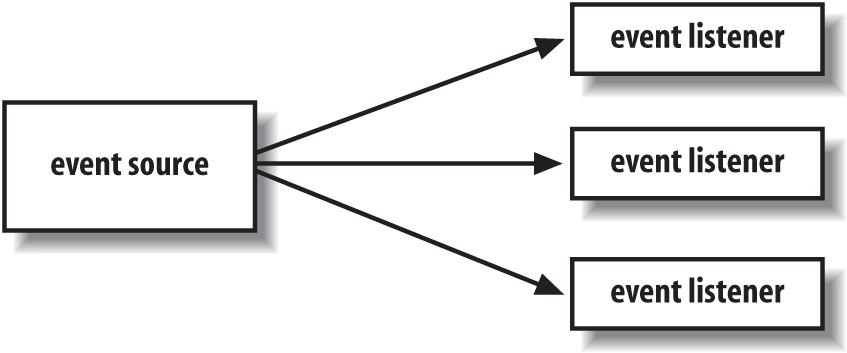
\includegraphics[width=1.0\textwidth]{Imagenes/Bitmap/Listener.png}
\caption{Patr\'on Listener}
 \label{Patron_Listener}
\end{figure}
\\
La librer\'ia realizada para este proyecto utiliza este patr\'on. Para esto se ha implementado una interfaz llamada \textbf{InputMobileInterface} que sirve para avisar al objeto que implemente dicha interfaz de:
\begin{itemize}
\item Recepci\'on de una pulsaci\'on por parte del usuario.
\item Valores del alto y ancho en pixeles de la pantalla del tel\'efono m\'ovil del usuario que se ha conectado.
\item Notificaci\'on del final de la conexi\'on.
\end {itemize}
Al tratarse una interfaz p\'ublica, cualquier clase puede convertirse en Listener de InputMobileInterface heredando de esta e implementando los 3 m\'etodos mencionados anteriormente. En el cap\'itulo siguiente se explicar\'a de manera m\'as detallada los pasos a seguir para la inclusi\'on de esta serie de scripts en un juego ya terminado junto con las pruebas con usuarios. La librer\'ia desarrollada consta de 3 scripts que se comunican entre si para realizar las funciones que se han descrito en este apartado.

\begin{figure}[h]
\centering
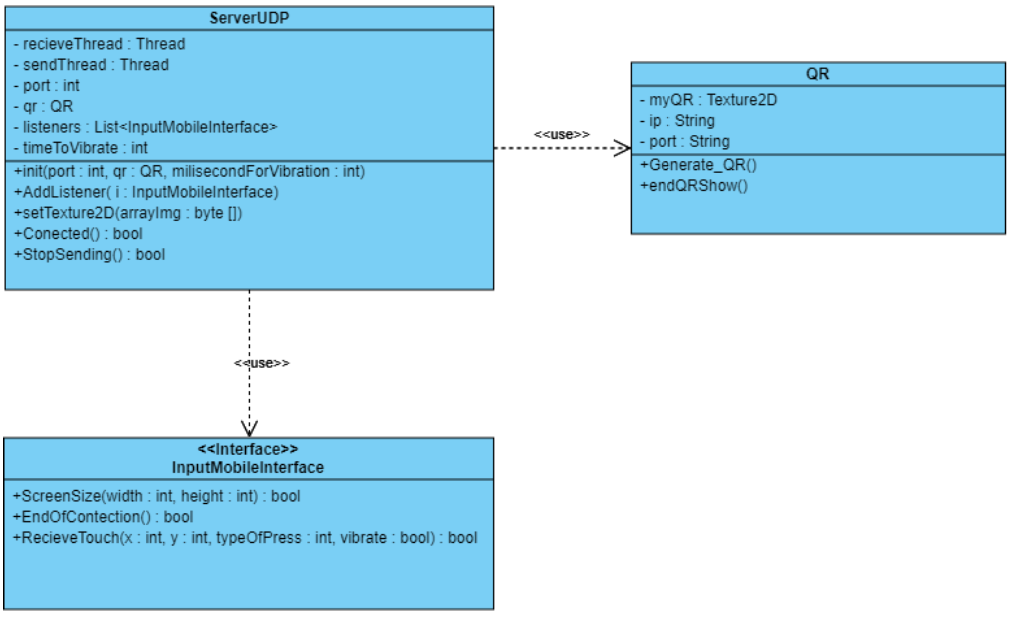
\includegraphics[width=1.0\textwidth]{Imagenes/Bitmap/Arquitectura_Unity.png}
\caption{Arquitectura de la librer\'ia implementada para Unity}
 \label{Unityr}
\end{figure}

La clase \textbf{ServerUDP} es la clase principal y es de la cual se requiere tener una instancia en el proyecto. Esta clase es la encargada de guardar y registrar listeners. Adem\'as se encarga de utilizar la clase \textbf{QR} que implementa la funcionalidad para generar el c\'odigo QR correcto con el uso de la librer\'ia ZXing.Net. Por \'ultimo, la clase ServerUDP tiene como  cometido la inicializaci\'on del socket y la de inicar los hilos de recepci\'on y env\'io de datos al dispositivo m\'ovil cuando este se conecte. Una vez lleguen los datos de las pulsaciones, esta clase tambi\'en se encarga de avisar a todos los listeners que se hayan registrado.

% Variable local para emacs, para  que encuentre el fichero maestro de
% compilaci�n y funcionen mejor algunas teclas r�pidas de AucTeX
%%%
%%% Local Variables:
%%% mode: latex
%%% TeX-master: "../ManualTeXiS.tex"
%%% End:
